\documentclass[border=10pt]{standalone}

\usepackage{tikz}
\usepackage{tikzsymbols}
\usetikzlibrary{calc,patterns,shapes.geometric}

\def\centerarc[#1](#2)(#3:#4:#5){\draw[#1] ($(#2)+({#5*cos(#3)},{#5*sin(#3)})$) arc (#3:#4:#5);}

\begin{document}
	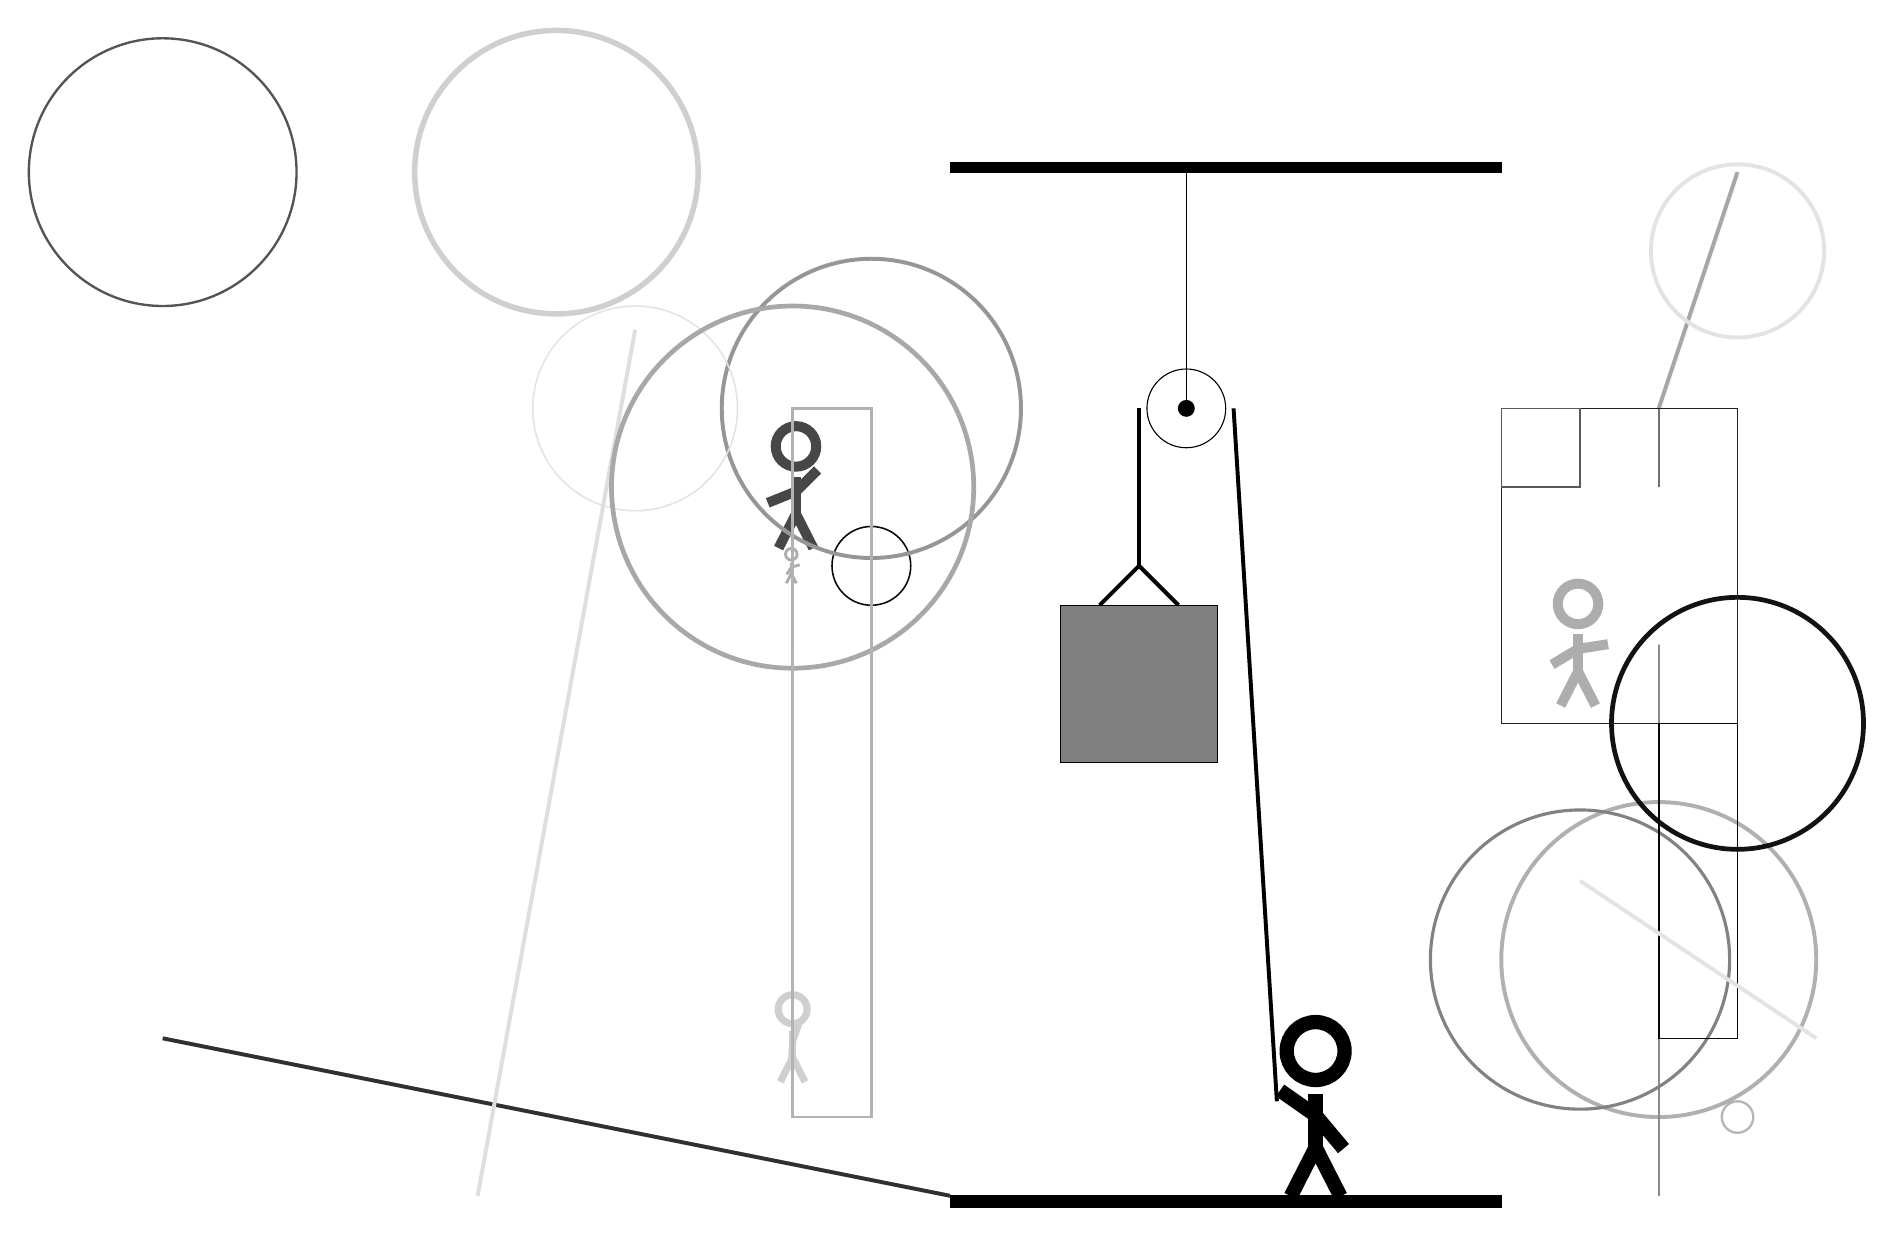
\begin{tikzpicture}
		%%%%% START %%%%%
		
		\draw[fill=black] (-2, 10) rectangle (5, 10.125);
		
		\draw (1, 7) circle (0.5);
		\draw[fill=black] (1, 7) circle (0.1);
		\draw (1, 10) -- (1, 7);
		
		\node[line width=0.2mm, color=black!19] at (-4, -1) {\Strichmaxerl[5][87][71]};
		
		\draw [line width=0.5mm, color=black!31](7, 0) circle (2.0);
		\draw [line width=0.7mm, color=black!19](-7, 10) circle (1.8);
		\draw [line width=0.2mm, color=black!96](-3, 5) circle (0.5);
		\node[line width=0.6mm, color=black!72] at (-4, 6) {\Strichmaxerl[7][22][45]};
		\node[line width=0.4mm, color=black!32] at (-4, 5) {\Strichmaxerl[2][58][15]};
		\node[line width=0.7mm, color=black!32] at (6, 4) {\Strichmaxerl[7][31][9]};
		\draw[line width=0.5mm, color=black!81](-2, -3) -- (-12, -1);
		\draw [line width=0.5mm, color=black!41](-3, 7) circle (1.9);
		\draw[line width=0.3mm, color=black!46] (7, -3) rectangle (7, 4);
		
		\draw[line width=0.3mm, color=black!56] (7, 7) rectangle (7, 6);
		
		\draw [line width=0.2mm, color=black!11](-6, 7) circle (1.3);
		\draw[line width=0.5mm, color=black!13](-6, 8) -- (-8, -3);
		
		\draw [line width=0.6mm, color=black!34](-4, 6) circle (2.3);
		\draw[line width=0.5mm, color=black!35](8, 10) -- (7, 7);
		\draw [line width=0.4mm, color=black!49](6, 0) circle (1.9);
		
		\draw[line width=0.3mm, color=black!30] (-3, -2) rectangle (-4, 7);
		\draw [line width=0.5mm, color=black!11](8, 9) circle (1.1);
		\draw [line width=0.6mm, color=black!93](8, 3) circle (1.6);
		\draw[line width=0.2mm, color=black!87] (5, 7) rectangle (8, 3);
		\draw [line width=0.3mm, color=black!67](-12, 10) circle (1.7);
		
		\draw [line width=0.3mm, color=black!29](8, -2) circle (0.2);
		\draw[line width=0.2mm, color=black!97] (7, -1) rectangle (8, 3);
		\draw[line width=0.5mm, color=black!11](9, -1) -- (6, 1);
		\draw[line width=0.2mm, color=black!29] (-4, 4) rectangle (-4, -2);
		
		\draw[line width=0.2mm, color=black!65] (6, 7) rectangle (5, 6);
		
		\draw[line width=0.5mm] (-0.1, 4.5) -- (0.4, 5.0) -- (0.9, 4.5);
		\draw[fill=black!50] (-0.6, 4.5) rectangle (1.4, 2.5);
		
		\draw[line width=0.5mm] (0.4, 7) -- (0.4, 5.0);
		\centerarc[line width=0.5mm](1, 7)(0:180:0.6);
		\draw[line width=0.5mm](1.6, 7) -- (2.15, -1.8);
		
		\node at (2.6, -1.9) {\Strichmaxerl[10][-35][-50]};
		
		\draw[fill=black] (-2, -3) rectangle (5, -3.15);
		
		%%%%% END %%%%%
	\end{tikzpicture}
\end{document}